\documentclass[a4paper, 12pt]{article}%тип документа

%отступы
\usepackage[left=0.6cm,right=1cm,top=2cm,bottom=3cm,bindingoffset=0cm]{geometry}
\setlength{\parindent}{5ex}

%Русский язык
\usepackage[T2A]{fontenc} %кодировка
\usepackage[utf8]{inputenc} %кодировка исходного кода
\usepackage[english,russian]{babel} %локализация и переносы

%Вставка картинок
\usepackage{graphicx}
\graphicspath{{pictures/}}
\DeclareGraphicsExtensions{.pdf,.png,.jpg}

%Графики
\usepackage{pgfplots}
\pgfplotsset{compat=1.9}

%Математика
\usepackage{amsmath, amsfonts, amssymb, amsthm, mathtools}

%Таблицы
\usepackage{longtable} 
\usepackage{float}

%Римские цифры
\newcommand{\RomanNumeralCaps}[1]{\uppercase\expandafter{\romannumeral#1}}

\usepackage{multirow}


\begin{document}
	\begin{titlepage}
		\begin{center}
			\textsc{Федеральное государственное автономное образовательное учреждение высшего образования«Московский физико-технический институт (национальный исследовательский университет)»\\[5mm]
			}
			
			\vfill
			
			\textbf{Отчёт по лабораторной работы 4.4.3\\[3mm]
				ИЗУЧЕНИЕ ЦЕНТРИРОВАННЫХ СИСТЕМ 
				\\[50mm]
			}
			
		\end{center}
		
		\hfill
		\begin{minipage}{.5\textwidth}
			Выполнил студент:\\[2mm]
			Сериков Василий Романович\\[2mm]
			группа: Б03-102\\[5mm]
			
		\end{minipage}
		\vfill
		\begin{center}
			Москва, 2023 г.
		\end{center}
		
	\end{titlepage}
	
	\newpage
	\textbf{Аннотация}\\
	
	
	\textbf{Цель работы: }\\
	Изучение методов определения фокусных расстояний линз и сложных оптических систем, а также изучить трубу Кеплера и с помощью метода Бесселя определить фокусные расстояния собирающих линз.\\
	
	\textbf{В работе используются: }\\ 
	 Оптическая скамья, набор линз, экран, осветитель со шкалой, зрительная труба, диафрагма, линейка.\\
	 
	 \textbf{Теоретические сведения: } \\
	 В данной работе мы будем проверять формулу тонкой линзы (a -- расстояние от предмета до линзы, b -- расстояние от линзы до изображения, F -- фокусное расстояние линзы): $$ \pm1/a \pm 1/b = \pm1/F $$
	 
	 Также будем определять фокусное расстояние линз с помощью метода Бесселя для случая, когда $n = n'$ и $f' = -f$. Тогда фокусное расстояние вычисляется по формуле:
	 \begin{equation}\label{Bessel}
	 	f = \frac{(L - \delta)^2 - l^2}{4(L-\delta)}.
	 \end{equation}
 
	\begin{figure}[H]
		\begin{center}
			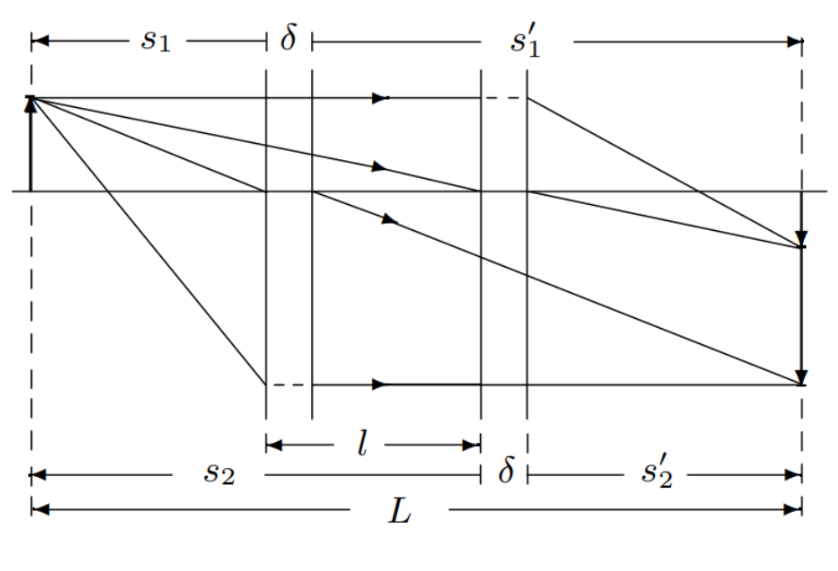
\includegraphics[width = 0.85\textwidth]{bessel.png}
			\caption{Метод Бесселя для центрированных систем}
		\end{center}
	\end{figure}
	
	\newpage
	
	\begin{figure}[H]
		\begin{center}
			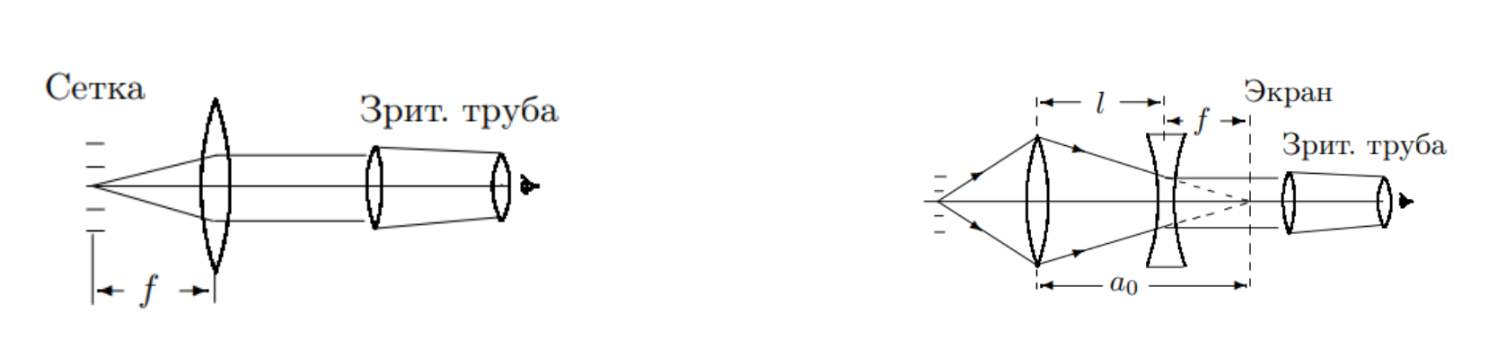
\includegraphics[width = 0.85\textwidth]{линзы.png}
			\caption{Методы определения фокусных расстояний линз с помощью зрительной трубы}
		\end{center}
	\end{figure}
	
	В данной работе предлагается собрать трубу Кеплера и установить, что коэффициент увеличения равен отношению фокусных расстояний первой и второй линз.
	
	\begin{figure}[H]
		\begin{center}
			\includegraphics[width = 0.85\textwidth]{kepler.png}
			\caption{Телескоп Кеплера из собирающих линз}
		\end{center}
	\end{figure}  

	\newpage
	
	\textbf{Ход работы и обработка результатов.}\\
	
	\begin{enumerate}
	
	\item Для проверки формулы тонкой линзы соберем схему с экраном и получим четкое изображение на нем, измерим расстояния от линзы до источника и от линзы до экрана: a, b соответственно. Полученные результаты занесем в таблицу 1. По результатам построим графики зависимости 1/b от (1/a) и ab = f(a + b)
	
	\begin{longtable}{|c|c|c|c|c|c|c|}
		\hline
		a, см & 37,7 & 14,1 & 12,5 & 59,1 & 15,4 & 30 \\ \hline
		b, см & 13,4 & 36,8 & 58,5 & 11,9 & 29,6 & 15,2 \\ \hline
		\caption{Результаты для первой линзы, $\sigma_{a,b} = \pm 0,2$ см}
	\end{longtable}
	
	\begin{longtable}{|c|c|c|c|c|c|c|}
		\hline
		a, см & 17,1 & 51,8 & 16,4 & 60,0 & 26,4 & 25,1 \\ \hline
		b, см & 52,1 & 17,4 & 60,1 & 16,6 & 24,7 & 26,0 \\ \hline
		\caption{Результаты для второй линзы, $\sigma_{a,b} = \pm 0,2$ см}
	\end{longtable}
	
	\begin{longtable}{|c|c|c|c|c|}
		\hline
		a, см & 24,5 & 50,7 & 21,5 & 72,4 \\ \hline
		b, см & 49.1 & 23,3 & 71,0 & 20,2\\ \hline
		\caption{Результаты для третьей линзы, $\sigma_{a,b} = \pm 0,2$ см}
	\end{longtable}
	
	\begin{figure}[H]
		\begin{center}
			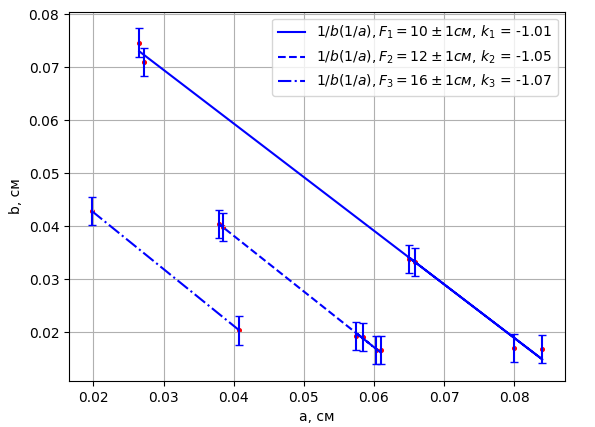
\includegraphics[width = 0.75\textwidth]{a(b).png}
			\caption{График зависимости 1/b(1/a) и расчет фокусного расстояния}
		\end{center}
	\end{figure}  
	
	
	\begin{figure}[H]
		\begin{center}
			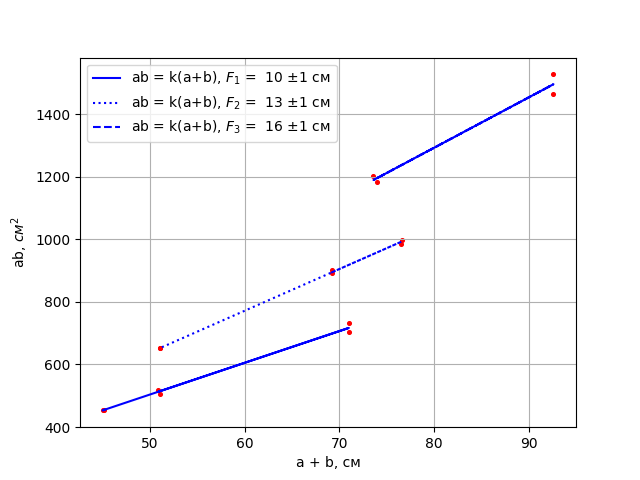
\includegraphics[width = 0.85\textwidth]{ab(a+b).png}
			\caption{График зависимости ab(a+b) и расчет фокусного расстояния}
		\end{center}
	\end{figure} 

	\item Проведем расчет фокусных расстояний линз с помощью зрительной трубки. 
	
	\begin{longtable}{|c|c|c|c|c|}
		\hline
		№ & 1 & 2 & 3 & 4 \\ \hline
		F, см & 10,4 & 13,1 & 15,1 & -10,6\\ \hline
		\caption{Фокусные расстояния, измеренные с помощью зрительной трубы, $\sigma_F = 0,2$ см}
	\end{longtable}
	
	\item Определим фокусные расстояния с помощью метода Бесселя
	
	\begin{longtable}{|c|c|c|c|}
		\hline
		№ & 1 & 2 & 3  \\ \hline
		F, см & 10,2 & 12,9 & 16,1 \\ \hline
		\caption{Фокусные расстояния, определенные с помощью метода Бесселя, $\sigma_F = 0,3$ см}
	\end{longtable}
	
	\textbf{Обсуждение результатов и выводы: }\\
	
	В данной работе мы изучили способы определения фокусных расстояний линз, из полученных результатов можно сделать вывод, что все способы эквиваленты.
	
	
	
	
	\end{enumerate}
	
	
	
	
	
	\end{document}